\documentclass[a4paper,11pt]{article}
\usepackage{graphicx}
\usepackage{booktabs}
\usepackage{setspace}
\usepackage{parskip}
\onehalfspacing
\begin{document}

\author{Hiromasa Okada}
\title{\vspace{-2cm}Report for Sheet 1\\
\small{Lab Course Machine Learning and Data Analysis}}
\maketitle
\section*{Implementation comments}

I have implemented PCA, AUC LLE and Gamma-index. AUC LLE and Gamma-index are simply implemented by functions but PCA is by class. If we create a PCA class with $pca = PCA(X)$ where $X$ is dataset with nxd (n is number of data points and d is the dimension of a data point), the programm saves  principle components and eigenvalue in objects. This class has two other functions $projection(self, X, m)$ and $denoise(self, X, m)$ where $m$ is number of dimension to which we will reduce. Projection is used for dimension reduction by using the saved principal components and denoise is used for denoising by reconstruction from the projected data points. \\
The function $auc(y_true, y_val, plot=False)$ where $ytrue$ is label array and $yval$ is value array returns AUC. If $plot$ is true it shows also ROC graph. \\
The function $lle(X, m, tol, n_rule='knn', k=5, epsilon=1.)$ returns in m dimension embedded data points. If a rule $knn$ is choosen, during the lle k-neighbors are choosen or if a rule $eps_ball$ is choosen, the neighbors in a distance "epsilon" are choosen.

By the test programm the principal components of PCA are not same as the $Ucorrect$ but my programm has the same result as the result of scikit-learn's principal components.

\begin{verbatim}
import sheet1 as imp
print("Principle conponents of my inplementaion")
pca = imp.PCA(X)
print(pca.U)
print("correct Principle conponents")
print(correct_U)
p= sklearn.decomposition.PCA()
p.fit(X)
aaa = -p.components_
print("Principle conponents by scikit-learn")
print(-p.components_)

Principle conponents of my inplementaion
[[-0.3655603   0.85514315 -0.36755389]
 [ 0.79651591  0.49171606  0.35182059]
 [-0.48158911  0.16415088  0.86088699]]
correct Principle conponents
[[ 0.3655603  -0.85514315  0.36755389]
 [-0.79651591 -0.49171606 -0.35182059]
 [-0.48158911  0.16415088  0.86088699]]
Principle conponents by scikit-learn
[[-0.3655603   0.85514315 -0.36755389]
 [ 0.79651591  0.49171606  0.35182059]
 [-0.48158911  0.16415088  0.86088699]]
\end{verbatim}


\section*{Assignment 5}
In this assignment, I analyzed the usps dataset with PCA.
\subsection*{1. Load the usps data set.}
With following code I loaded data set X (nxd) where d is dimension and n is number of data points.
\begin{verbatim}
from scipy.io import loadmat
#1. Load the usps data set.
data = loadmat('usps.mat') 
label = data['data_labels']
pat = data['data_patterns']
\end{verbatim}
\subsection*{2. Analysis of PCA}

But to be accepted, X must be transposed before calicurating PCA.
\begin{verbatim}
#2. Analysis of PCA:
pca = imp.PCA(pat.T)
\end{verbatim}
Now princile components are calicurated.
Next visualize all principal values, the largest 25 principal values and the first 5 principal directions.

\begin{verbatim}
#(a) Visualize all principal values,
plt.figure(0, (16,4))
cut = len(pca.D)
plt.bar(np.arange(cut), pca.D[:cut], lw=0)
plt.title("eigenvalues")
plt.show()

#(b) Visualize the largest 25 principal values 
plt.figure(0, (16,4))
cut = min(len(pca.D),25)
plt.bar(np.arange(cut), pca.D[:cut], lw=0)
plt.title("eigenvalues")
plt.show()
\end{verbatim}

\begin{figure}[htbp]
  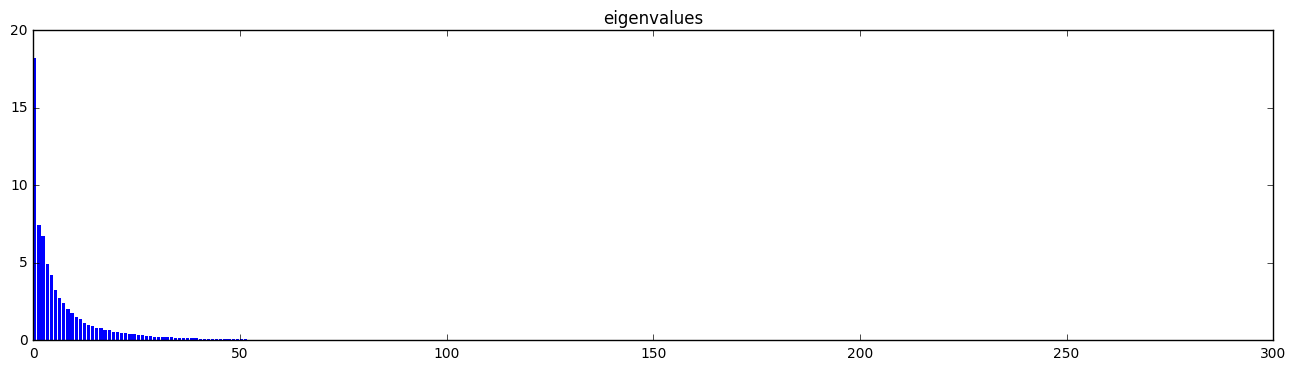
\includegraphics[scale=0.4]{allpc.png}
  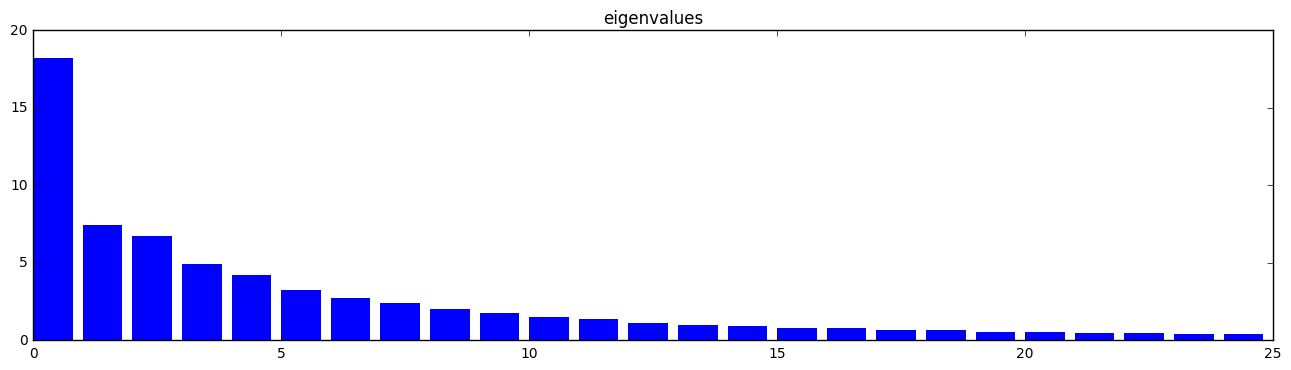
\includegraphics[scale=0.4]{5pc.png}
\end{figure}

\begin{verbatim}

\end{verbatim}

From these graphs we know the first largst principal value is much larger than second largest value and following. It means that the principal direction with the largest principal value is the most correlated direction. Principle value means also variance so that it shows this direction is the largest.  \\ 

\begin{verbatim}
#(c) the first 5 principal directions (as images, see imshow).
plt.figure(figsize=(48,32))
for i in range(5):
    plt.subplot(16,16,i+1)
    plt.title("eigenvector %i" % (i+1))
    plt.imshow(pca.U.T[:,i].reshape(16,16))
\end{verbatim}


\begin{figure}[htbp]
  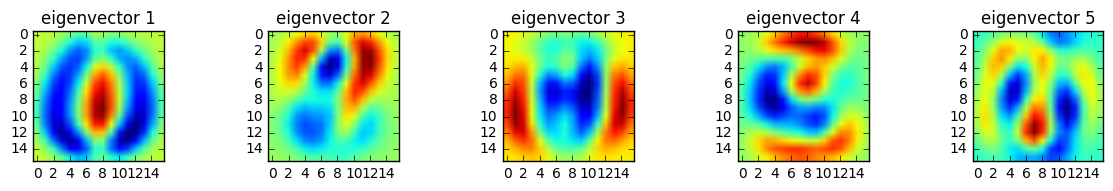
\includegraphics[scale=0.4]{5eigv.png}
  \caption{First 5 Principle directions}
\end{figure}

\subsection*{3. Consider three noise scenarios}
First I made noised images and an example is following. Each noise is produced by $numpy.random.randn$ and for Weak noise variance=0.1, for strong noise variance=0.3 and extream noise variance = 1.8.
\begin{figure}[htbp]
  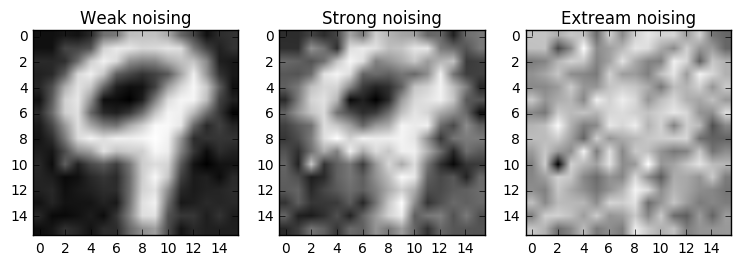
\includegraphics[scale=0.4]{noisimg.png}
  \caption{Example of a noised image}
\end{figure}

\ After PCA computation I got following values of principal palues. \\
From this results we know that small principal values are differ from each others but large values are almost same. Therefore large value corresponding principal direction has features of original data and small value corresponding principal values shuld be noises.
\begin{figure}[htbp]
  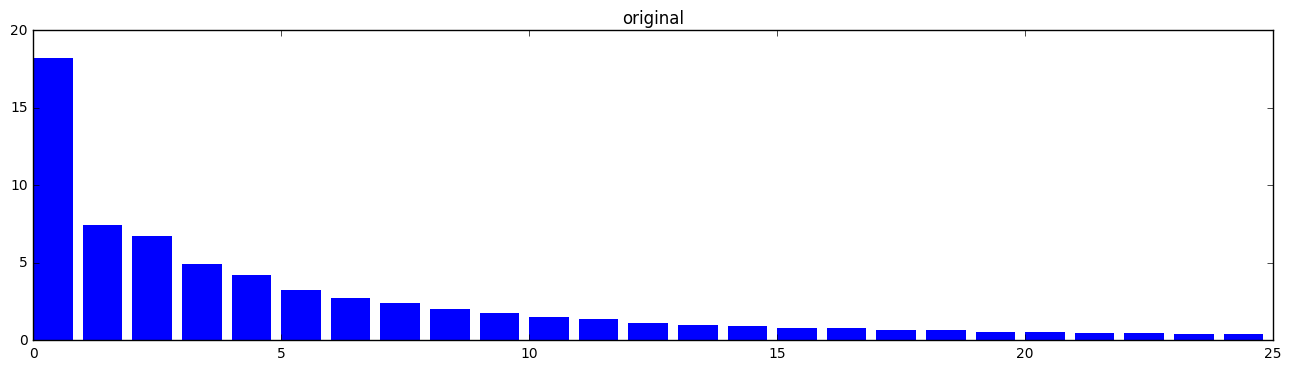
\includegraphics[scale=0.4]{orgev.png}
  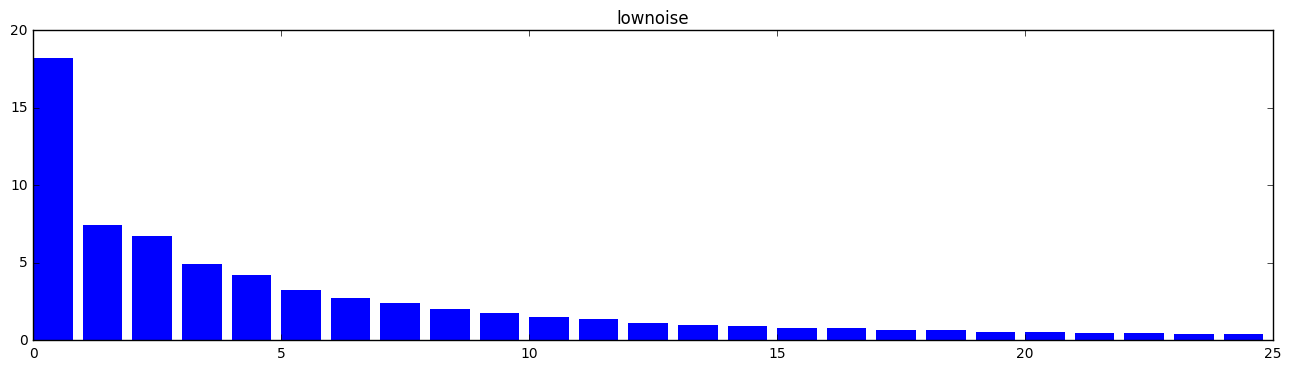
\includegraphics[scale=0.4]{lowev.png}
  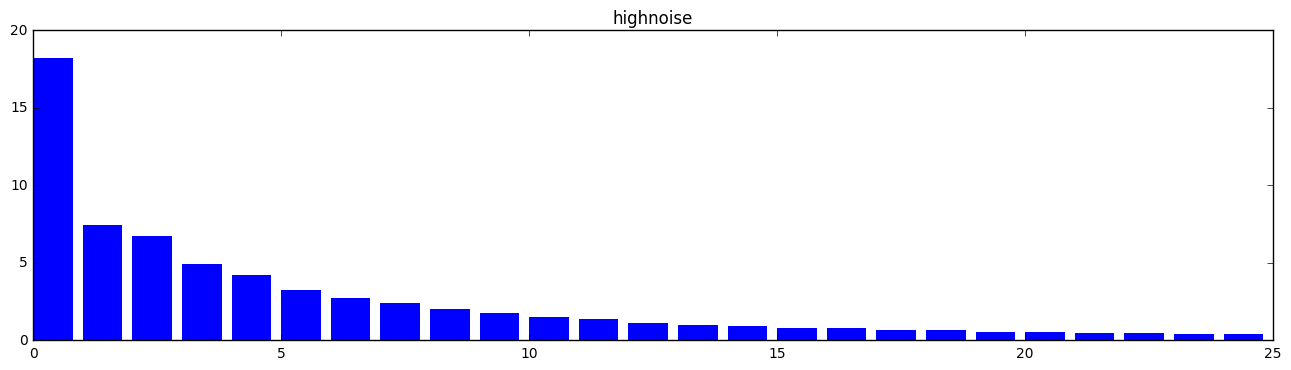
\includegraphics[scale=0.4]{stev.png}
  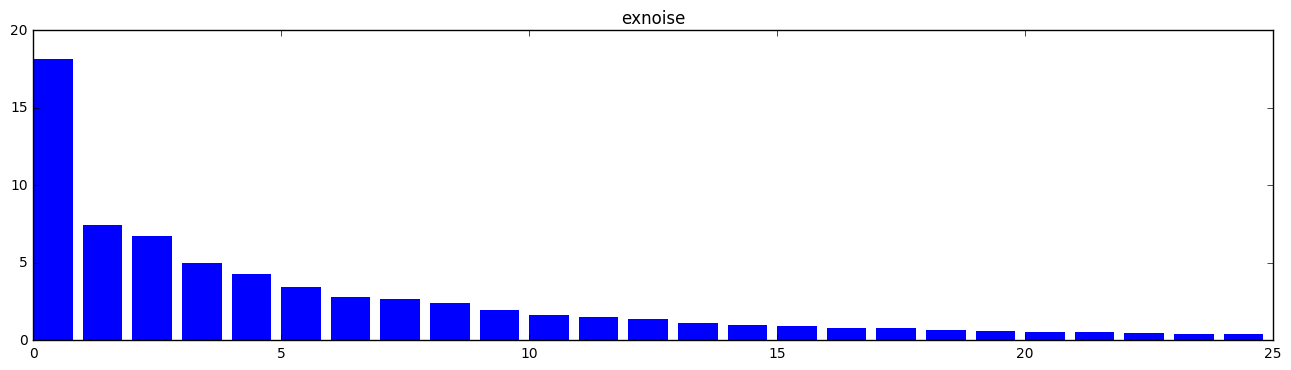
\includegraphics[scale=0.4]{exev.png}
  \caption{Example of largest 5 principle values}
\end{figure}

\begin{figure}[htbp]
  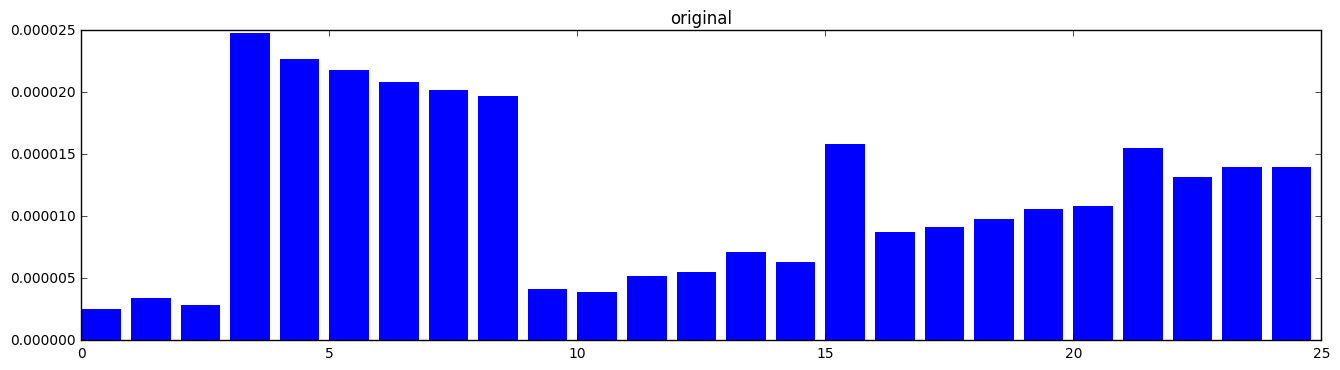
\includegraphics[scale=0.4]{orgev2.png}
  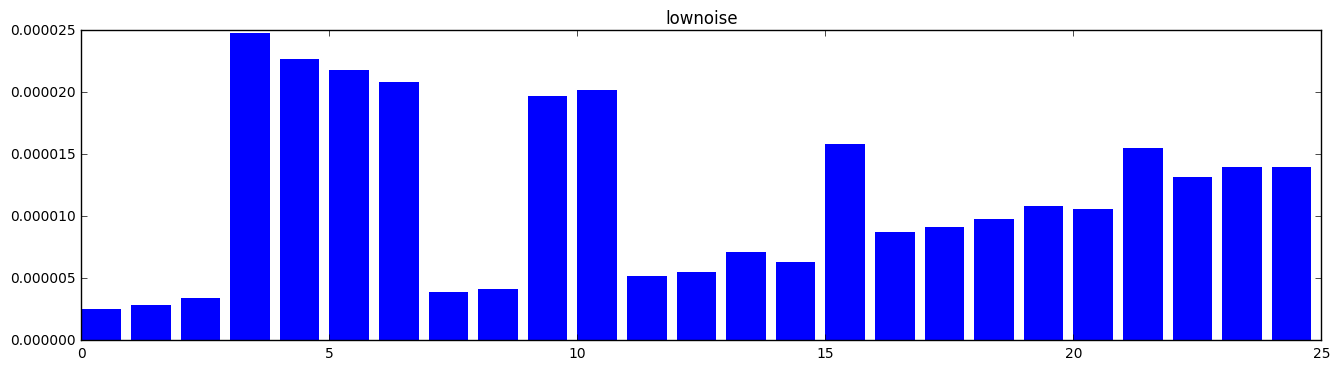
\includegraphics[scale=0.4]{lowev2.png}
  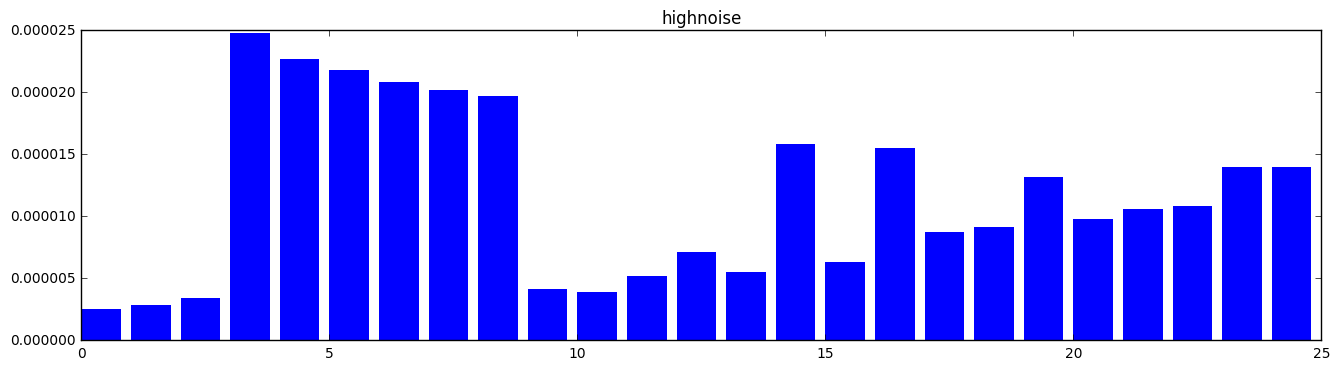
\includegraphics[scale=0.4]{stev2.png}
  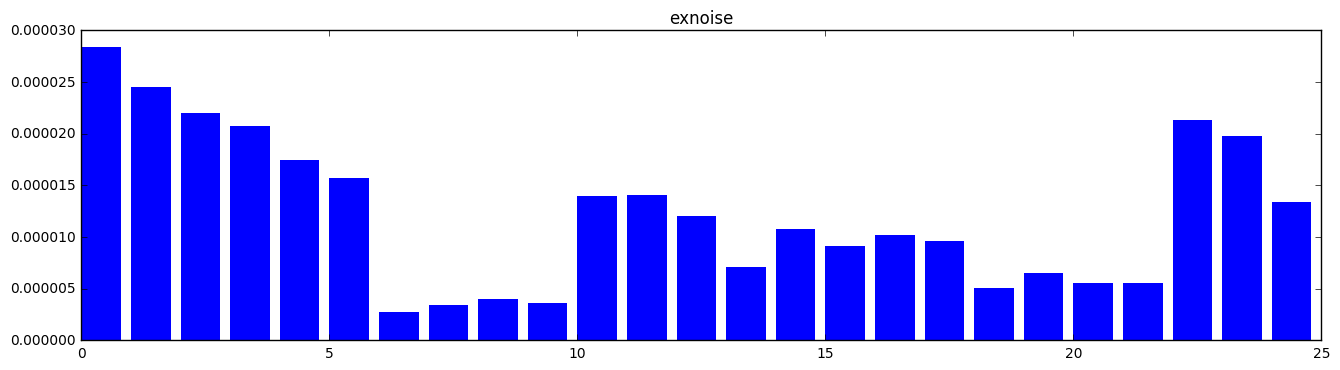
\includegraphics[scale=0.4]{exev2.png}
   \caption{Example of smallest 5 principle values}
\end{figure}
\subsection*{4. Define m}
~Now I'd like to find the number $m$ how many principal components are used for denoising. For each noise case, to find m I tried from m=1 to m=100 and calicurated average errors between reconstructed points and original data points. The error in case of weak noise decreased fast until m=40 with error= 9.274096 and then slowly decreased until m=81. After that the error went up slowly. So in this case I choosed m=81. The error in case of strong noise decrease fast until m=41 with error= 9.549555 and then increased faster than case of weak noise. Errors of strong noise case were always larger than weak noise case.

\begin{figure}[htbp]
  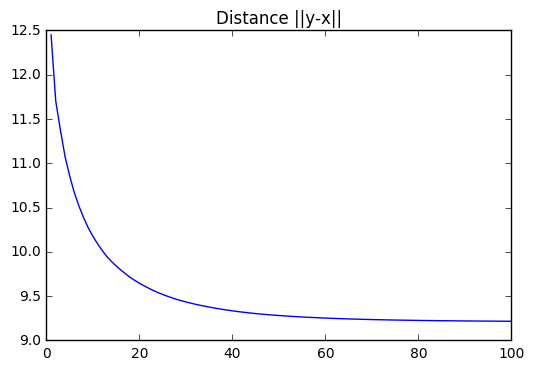
\includegraphics[scale=0.7]{dlown.png}
  \caption{Distance between original and from lownoise reconstructed}
   \end{figure}
\begin{figure}[htbp]
  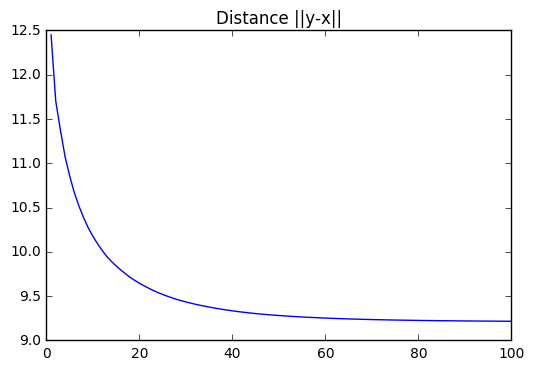
\includegraphics[scale=0.7]{dh.png}
  \caption{Distance between original and from strong noise reconstructed}
  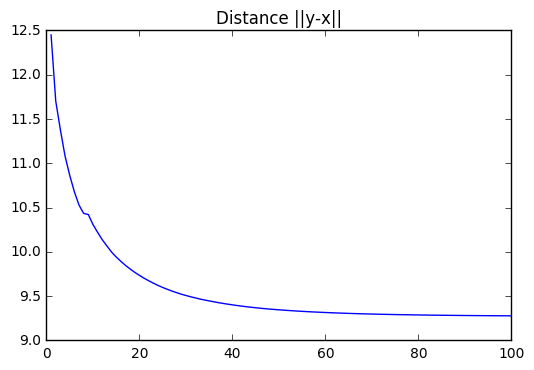
\includegraphics[scale=0.7]{de.png}
  \caption{Distance between original and from extream noise reconstructed}
\end{figure}

\begin{verbatim}







\end{verbatim}

\subsection*{5. Denoising Images}
~~For 10 examples of choices, plot the
original image, the noisy image and its denoised reconstruction. \\
~~After reconstruction of noised images, the images with weak noise and strong noise were reconstructed very well. Reconstructed images look like blured images. But images with extream noise were not reconstructed. Too strong noise washes out original data so that these are not to be reconstructed.
\begin{figure}[htbp]
  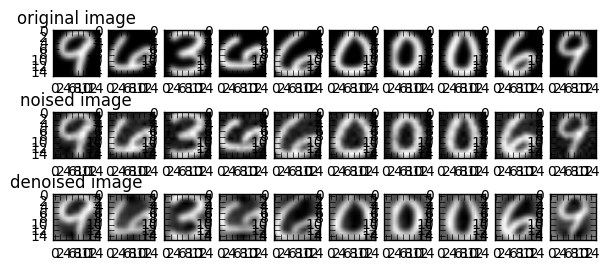
\includegraphics[scale=0.7]{ld.png}
  \caption{Low noise 10 examples comparing to original and denoised}
  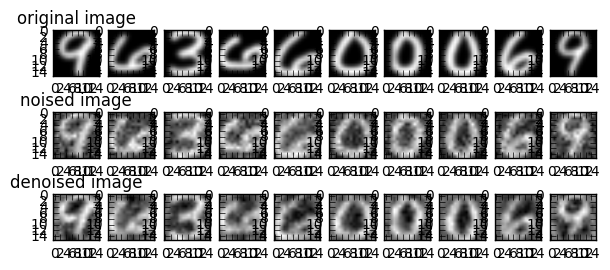
\includegraphics[scale=0.7]{sd.png}
  \caption{Strong noise 10 examples comparing to original and denoised}
  \end{figure}
\begin{figure}[htbp]
  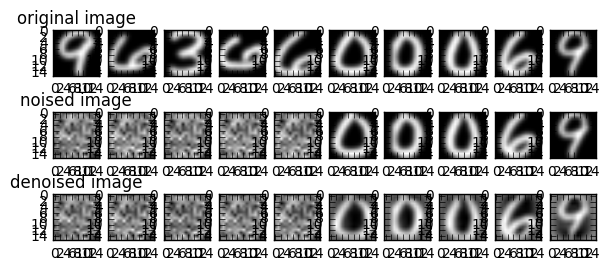
\includegraphics[scale=0.7]{ed.png}
  \caption{Extream noise 10 examples comparing to original and denoised}
  \end{figure}
  
\begin{verbatim}








\end{verbatim}
  
  
  
\section*{Assignment 6}
\subsection*{1. Choosing a randam set of outliers}
\ I choosed randomly outliers from the negative class of the respective size (depending on the
outlier rate). A following code is an example of choosing outliers and calicurate gamma index with k=3 and k=10 in case of outlier rate 1 percent.

\begin{verbatim}
p = np.array([0.01, 0.05, 0.1, 0.25])
N = len(data[0])
NN = len(negclass[0])
NP = len(posarg[0])
n = NP*p/(1-p)

choice1 = np.random.choice(NN,int(n[0]))
negchoiced1 = negclass[:,choice1]
newset1 = np.append(inlines, negchoiced1,axis=1)
gammak3_1p[i] = imp.gammaidx(newset1.T, 3)
gammak10_1p[i] = imp.gammaidx(newset1.T, 10)
\end{verbatim}

\subsection*{2. Calculating Gamma Index}
Above code was itarated 100 times and calicurated avarage of gamma index.
\begin{figure}[htbp]
  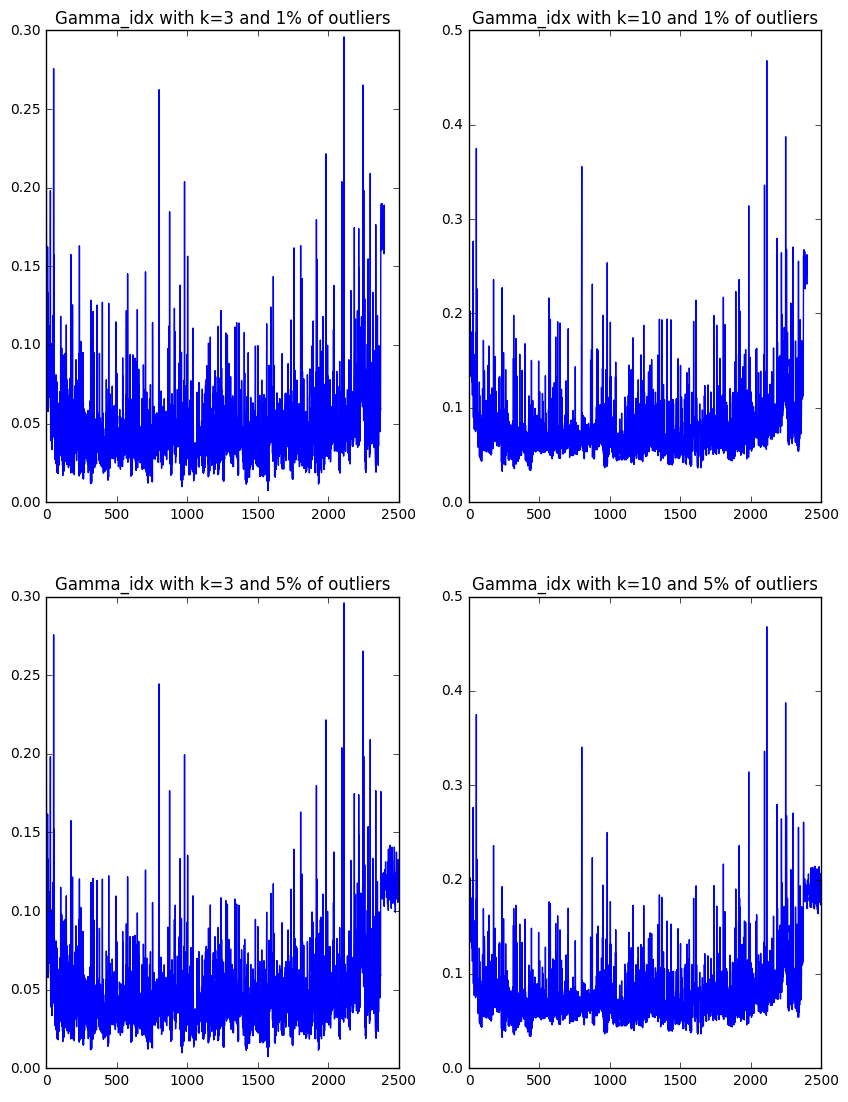
\includegraphics[scale=0.5]{index1.png}
\end{figure}
\begin{figure}[htbp]
  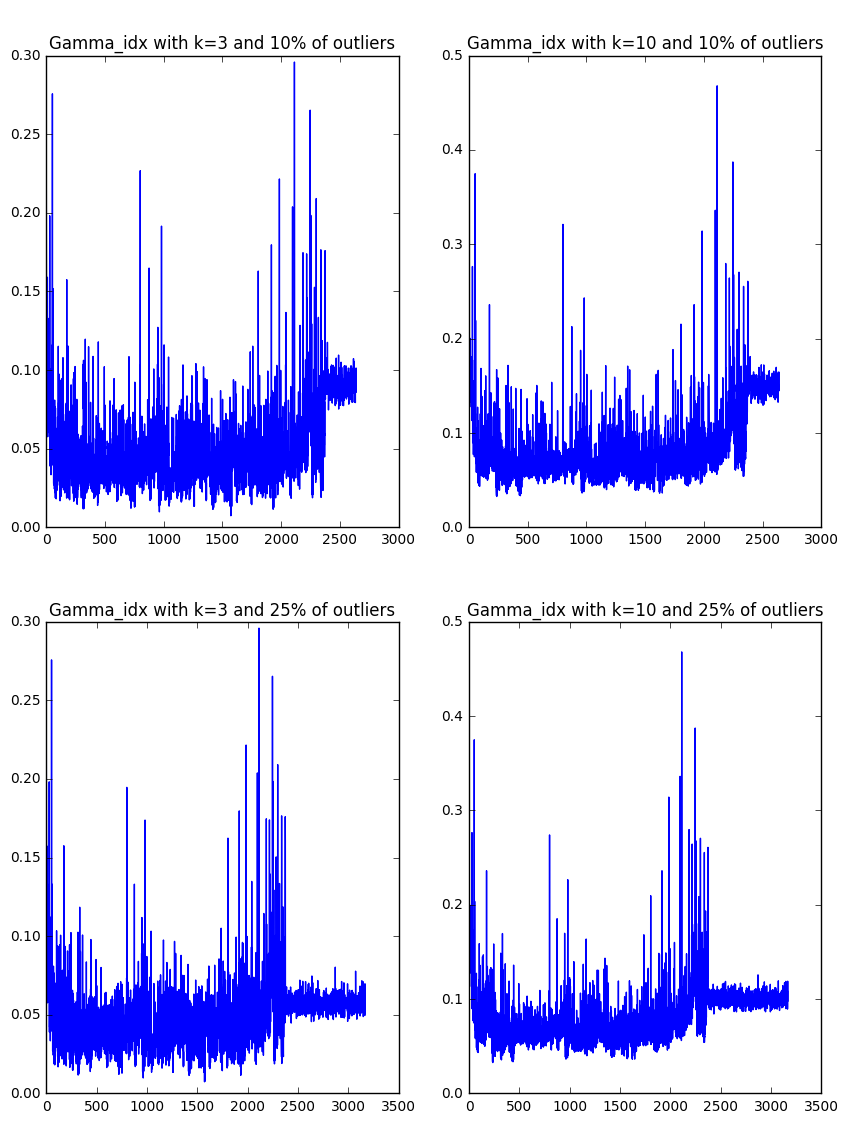
\includegraphics[scale=0.5]{index2.png}
\end{figure}

\begin{verbatim}






\end{verbatim}
\ For 1 percent of outliers outliers have long mean distances bitween others(outliers are at the end of graphs because outliers were simply added after inliers) because if outliers are few, outliers have to choose some inliers as neighbors. On the other hands if there are more outliers, the outliers have other outliers as neighbors. Therefore mean distances of outliers for 10 percent and 25 percent are much shorter. And for each case gamma index is larger with k=10 than with k=3. This means if we set more neighbors, mean length between the point and neighbors are longer.

\subsection*{3. Calculating AUC}
\ In this case AUC means the area of ROC which is computed by thresholding of defferent dinstances. To find the AUC, I found the mean point and distances between each point and the mean point. Then I inversed these distances and sorted. By setting a Threshold for distances each point is predicted as "inlier" or "outlier". If inversed distance is over the Threshold, it shuld be a "inlier" otherwise "outlier". Following is the Algorithum in case of 1 percent of outliers.

\begin{verbatim}
mpoint1 = np.mean(newset1,axis=1)
D1 = np.linalg.norm(newset1-mpoint1.reshape(2,1),axis=0)
D1[np.where(D1==0)] = np.min(D1)
invD1 = 1/D1
c[0][i] = imp.auc(newlabel1, invD1, plot=False)
\end{verbatim}

And then plotted box plot.

\begin{verbatim}
#Boxplot(C)
plt.boxplot(c.T)
plt.xticks([1, 2, 3,4],['1%','5%','10%','25%'])
\end{verbatim}

\begin{figure}[htbp]
  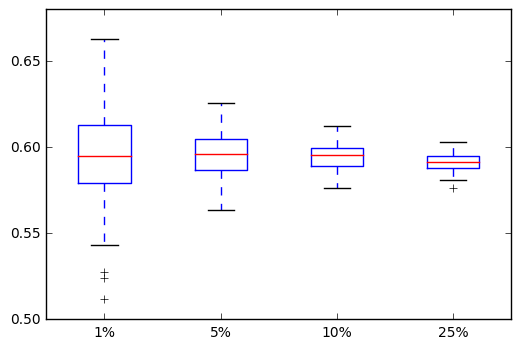
\includegraphics[scale=0.5]{auc.png}
  \caption{Boxplot of the AUC}
\end{figure}

\begin{verbatim}






\end{verbatim}


\ From this graph we know that if we have less outliers the variance of AUC will be bigger and vice versa. In every case mean has almost no defference.



\section*{Assignment 7}
\subsection*{1. Plot the 3D data}
\begin{figure}[htbp]
  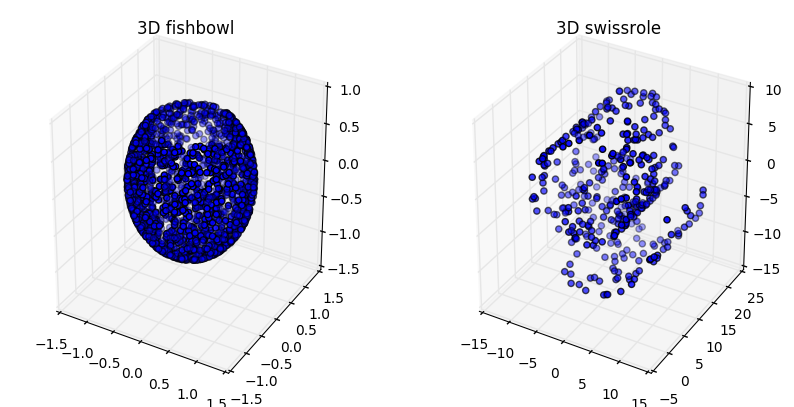
\includegraphics[scale=0.5]{3d.png}
\end{figure}
There 3D plot of the dataset fishball and swissroll. These 2 dataset are embedded in 2D space.
\begin{verbatim}





\end{verbatim}
\subsection*{2. Plot the 2D and 1D embedded data}
\begin{figure}[htbp]
  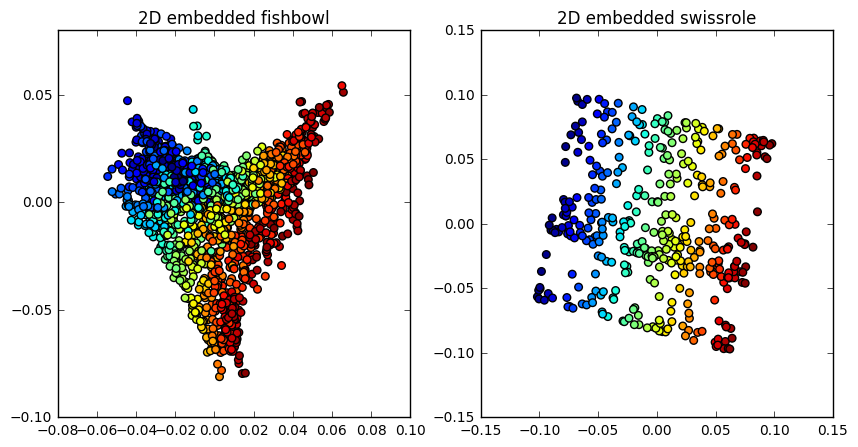
\includegraphics[scale=0.5]{2d.png}
\end{figure}
To plot the 2D embedded data I used lle which I implemented and used "epsilon ball rule" with $tol=1e-10$ and $epsilon=0.14441549$ for the fish ball data set and "knn" with $tol=1e-4$ and $k=8$ for the swissroll data set.
 
\begin{verbatim}
fishlle = imp.lle(fish.T, m=2, tol=1e-10, n_rule='eps-ball', k=15,\
 epsilon=0.14441549)
srlle = imp.lle(sr.T, m=2, tol=1e-4, n_rule='knn', k=8, epsilon=0.1)
\end{verbatim}
By several tries these configlations were found and I noticed that for uniformaly concentrated data set like fish ball epsilon ball is suitable and for non uniformaly sparse data like set swissroll knn is more suitable. \\
\ 2D data set can be also embedded. 
\begin{verbatim}
frlle = imp.lle(fr.T, m=1, tol=1e-06, n_rule='knn', k=15, epsilon=0.1)
\end{verbatim}
\begin{figure}[htbp]
  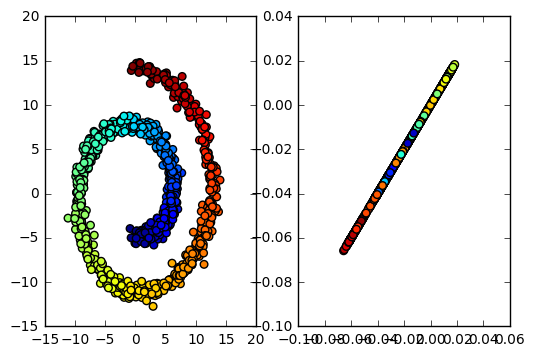
\includegraphics[scale=0.5]{2d1d.png}
  \caption{2D flatroll and 1D embedded plot}
\end{figure}

\section*{Assignment 8}
\subsection*{1. Influence of noise on LLE}

\end{document}



